\chapter{The Global Data Plane}
\label{gdp}

We have developed Secure Content Distribution Trees in conjunction with the Global Data Plane (GDP) project. The SCDT concept is not exclusive to the GDP; however, the GDP is a case study of the applications benefited by SCDTs. We will reference the GDP throughout the remainder of this paper in order to demonstrate the broader  infrastructure SCDTs are designed to operate within.

\section{GDP Architecture for the Internet of Things}
\label{gdp-arch}
\begin{figure}[t]
	\begin{center}
		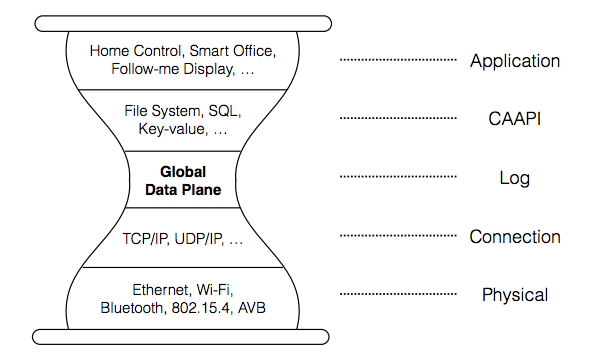
\includegraphics[scale=0.75]{gdp_stack.png}
	\end{center}
	\vspace{-1.3em}
	\caption{\small \itshape  The Global Data Plane (GDP) operates above the network level and offers Common Access APIs (CAAPIs) to applications rather than raw packet routing. We argue that this abstraction is more appropriate for both IoT applications and the cloud.}
	\vspace{-1em}
	\label{fig:gdp_stack}
\end{figure}

The Global Data Plane (GDP) is a data-centric abstraction
focused around the distribution, preservation, and
protection of information \cite{kubi}. It supports the same application
model as the cloud, while better matching the needs
and characteristics of the IoT by utilizing heterogeneous
computing platforms, such as small gateway devices, moderately
powerful nodes in the environment and the cloud,
in a distributed manner.
As shown in~\autoref{fig:gdp_stack}, the GDP interface provides a new
“narrow waist” upon which applications are constructed.
The basic foundation of the GDP is the secure, singlewriter
log. Logs in the GDP are lightweight, durable,
and they support multiple simultaneous readers—either
through random access (pull-based) or subscription (push-based).
Logs have no fixed location but rather are migrated
as necessary to meet locality, privacy, or QoS needs
of applications.
Applications are built on top of the GDP by interconnecting
log streams, rather than by addressing devices or
services via IP. Each sensor or computational element of
an IoT application has its own unique output log in the
GDP and writes timestamped entries to this log. Actuators
read from a unique input log. The GDP masks the
heterogeneity of underlying communication paradigms,
network/storage devices, and physical connections; and
on top, it supports a wide variety of Common Access Application
Program Interfaces (CAAPIs) for applications.
We detail a few key design decisions below:

\textbf{1. Single-writer time-series logs:} For each IoT device
or application component that generates data, this data is
represented as a log where the owner has the sole write
permission. This model is based on our observation that
peripherals are physical devices in our environment. We
assume that devices have cryptographic keys for signing
and encryption. Logs are append-only; most data is readonly
and can be securely replicated and validated through
cryptographic hashes.
For each log, our current design exposes append, read
and subscribe APIs. The single-writer model allows the
following properties:

\begin{itemize}
\item \textit{Flexibility:} The log interface is minimum but complete.
Aggregations of logs or CAAPIs (discussed below) can
be built by composition. In part (a) of~\autoref{fig:gdp_log}, a new log
is created by composing two existing ones and writing
back to the GDP.
\item \textit{Access Control:} Since devices and services have associated
public-key identities, each log has a single authorized
writer. An append operation is permitted only
when signed by the appropriate writer’s key. For read
operations, only those with an appropriate decryption key can decrypt the data, providing for a way to implement
read-access control policies; a variety of more
complex access control policies can be constructed
through hierarchical key management or selected use
of trusted environments.
\item \textit{Authenticity and integrity:} Since only signed append
operations are allowed, accidental or malicious corruption
of the log won’t occur and substitution attacks are
easily detected. A variety of traditional consistency
problems are replaced with the simpler problem of
finding the latest update.
\item \textit{Encryption:} We envision that all data written to the log
is encrypted with the encryption key held by the writer.
A single writer with a single encryption key simplifies
the key management challenges.
\item \textit{Durability and replication:} In contrast to the cloud
where users rely on whatever durability the cloud
providers offer, our model enables the choice of the
level of durability and geographic span of replication
on a per log basis. The log model also simplifies
replica consistency as previously mentioned.
\end{itemize}

\textbf{2. Location-independent Routing:} Logs must be physically
stored in the infrastructure. As previously discussed,
the current reliance of IoT on cloud storage provides
few guarantees about the placement, latency of access,
or durability of information. Instead, to embrace heterogeneous
platforms and support a variety of storage
policies, the GDP employs location-independent routing
in a large, 256-bit address space. To meet the goal of
flexible placement, controllable replication and easy migration,
packets are routed through an overlay network
that uses Distributed Hash Table (DHT) technology. DHT
addresses the challenges of scalability \cite{pastry, chord, tapestry} with
the sacrifice of an increased number of overlay hops. GDP
optimizes latency through log migration (see~\autoref{fig:gdp_log}(d))
and dynamic changes to the routing topology.

Logs are named with a 256-bit identifier which may be
derived from a cryptographic hash of the owner’s public
key and metadata. Following a variety of placement and
replication policies,
the GDP places logs within the infrastructure
and advertises the location of these logs to the
underlying routing layer. Such placement and replication
policies can optimize for latency, QoS, privacy, durability,
and so forth. Internally, logs are further split into chunks,
and each chunk can be distributed for durability \cite{oceanstore} and
performance \cite{bolt} (see~\autoref{fig:gdp_log}(b)).

\begin{figure}[t]
	\begin{center}
		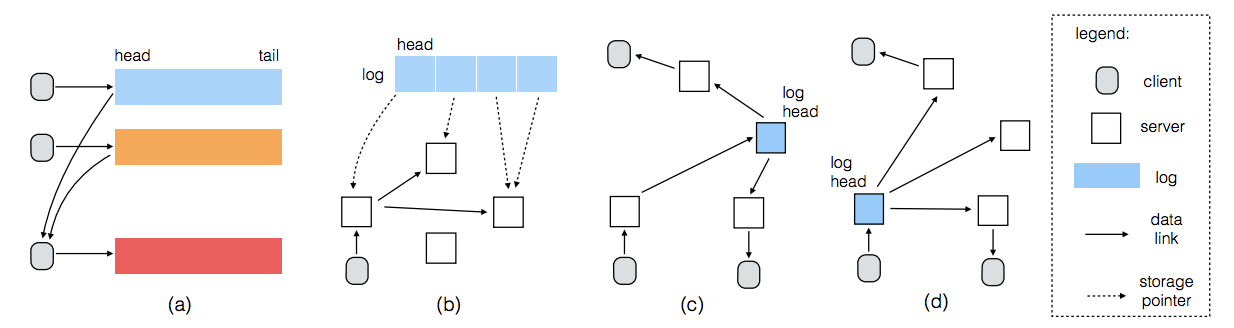
\includegraphics[scale=0.75]{gdp_log.png}
	\end{center}
	\vspace{-1.3em}
	\caption{\small \itshape  The GDP design illustrated: (a) single-writer logs are appended to the head and compositions are achieved by subscription;
		(b) logs are split into chunks and stored in a distributed fashion; (c) overlay multicast trees are constructed when there are multiple
		subscribers; (d) location-independent routing enables log migration for optimizing performance.}
	\vspace{-1em}
	\label{fig:gdp_log}
\end{figure}

\textbf{3. Pub/Sub and multicast tree:} The publish/subscribe
pattern has been shown to support a wide variety of fundamental
communication services (for mobility, multicast,
anycast \cite{indirection}). This fits nicely with our log abstraction
and can support building interactive applications. To
alleviate the growth of sensor data bandwidth, when multiple
subscribers exist, multicast trees can be built on top
of the overlay network using techniques proposed earlier \cite{cbt, tapestry} so that effective bandwidth is reduced \cite{end-system-mc} 
(see~\autoref{fig:gdp_log}(c)).

\textbf{4. Common Access API (CAAPI):} Although the singlewriter
log abstraction shelters developers from low-level
machine and communication primitives, many applications
are likely to need more common APIs or data structures
\cite{tango}. In fact, logs are sufficient to implement any
convenient, mutable data storage repository. Thus, ~\autoref{fig:gdp_stack}
shows a CAAPI layer on top of the GDP. A CAAPI can
provide key-value store, file system or database operations.
Since logs serve as the ground truth, the benefit
of consistency, durability, scalability and availability are
carried over to CAAPIs for free. However CAAPIs may
need to replay the logs if the service fails; in this case,
checkpointing can be employed to avoid expensive log
replay.

Our design for the GDP is not yet bullet-proof and our
initial implementation has not withstood the test of widescale
deployment. Nonetheless, we believe that the
core concepts of the GDP overcome many IoT pitfalls in the following ways: the single-writer, append only
log models sensor data more accurately; integrity
and authentication by design provides better privacy and
security; the distributed nature with peer-to-peer technology
makes scalability possible; explicit separation of
policy from mechanism enables better control on level of
durability for end users; and finally, latency, bandwidth
and QoS guarantees are enabled by the integration of the
cloud and the local infrastructure.

\section{Secure Content Distribution Trees in the GDP}
\label{gdp-scdt}
The Global Data Plane Infrastructure and its pub/sub architecture offer a real-world case study for the application of Secure Content Distribution Trees (SCDTs), a networking protocol we will detail in the following chapters. SCDTs provide three main utilities to the GDP:

\begin{enumerate}  
	\item SCDTs provide the mechanism by which data is distributed to thousands or millions of geographically-disparate subscribers securely (and reliably, if necessary).
	\item SCDTs provide the mechanism for distributing data among durable replicas.
	\item SCDTs support fast distribution of data to local subscribers, enabling latency-dependent applications.
\end{enumerate}

The GDP is designed to allow publishers to reach thousands or millions of subscribers. Often, the publisher and many (or all) of the subscribers are low-powered IoT devices. Those requirements necessitate a multicast scheme; a traditional client-server model is simply not scalable. Because the GDP is designed to support many different applications, it also requires reliable distribution of published data. Even ignoring reliable applications, durable replicas require reliability support.

One of the major, distinctive features of the IoT in general and the GDP in particular is the peer-to-peer nature of many applications. For instance, a street intersection might have many ``smart" devices that need to communicate amongst themselves with strong latency constraints (such as stop lights, street cameras, and car sensors) and with devices further away with weaker latency requirements (such as nearby intersections or a central control) in a city's traffic control system (see~\autoref{fig:architecture}). A traditional client-server model would require round trips to the cloud; one of the design goals of the GDP and SCDTs is to break out of this model to focus on supporting edge computing.

